\section{Analysis}

\subsection{Analytical}

This section will detail the time complexity of each method.\\

\begin{table}[!htbp]
\centering
\begin{tabular}{| l | l |}
	\hline
	\textbf{Method} & \textbf{Time complexity} \\ \hline
	\code{isEmpty()} & O(1) \\ \hline
	\code{contains(Object)} & O(log n) \\ \hline
	\code{hasPredecessor(Object)} & O(1) \\ \hline
	\code{hasSuccessor(Object)} & O(1) \\ \hline
	\code{predecessor(Object)} & O(log n) \\ \hline
	\code{successor(Object)} & O(log n) \\ \hline
	\code{min()} & O(1) \\ \hline
	\code{max()} & O(1) \\ \hline
	\code{add(Object)} & O(log n) \\ \hline
	\code{delete(Object)} & O(log n) \\ \hline
	\code{iterator()} & O(1) \\ \hline
	\code{iterator(Object)} & O(log n) \\ \hline
	\code{toString()} & O(n) \\
	\hline
\end{tabular}
\caption{Summary of time complexity of each method.}
\end{table}

Red-black trees have five main properties:
\begin{enumerate}
\item A node is either black or red.
\item The root node is black.
\item Every leaf node is black.
\item A red node has black children.
\item Every path from a node to a leaf descendent contains the same number of black nodes.
\end{enumerate}

Since the height of the tree is referenced in demonstrating the time complexity of almost every method in the class, I first prove that the following limit on the height of a red-black tree \parencite{clrs}:
\begin{equation*}
h \leq 2\log_2(n+1)
\end{equation*}
\begin{proof}
To begin, we prove that a subtree with root node $n$ has a minimum of $2^{h_b(n)} - 1$ internal nodes (where $b_h(n)$, the 'black-height' of $n$, is the number of black nodes on any path from the node $n$ to any leaf, not including $n$): we do this by induction. For the base case - if the black height of $n$ is zero, then $n$ must be a leaf - and so $2^0 - 1 = 0$ is the number of internal nodes. So it holds for $b_h(n) = 0$. Now we assume that a node $n$ has a positive height and two children (i.e. $n$ is an internal node). Then each child must have a height of $b_h(n)$ or $b_h(n) - 1$, depending on the colour of the child. We can then apply the inductive hypothesis to the children - then each child has $2^{b_h(n) - 1} - 1$ internal nodes. Therefore we can simply sum the number of internal nodes of the two child subtrees to prove the claim - the subtree rooted at $n$ will have at least $(2^{b_h(n) - 1} - 1) + (2^{b_h(n) - 1} - 1) + 1 = 2^{b_h(n)} - 1$ internal nodes.

With the above combined with red-black tree properties, we can complete the proof: if we have a tree of height $h$, then according to the fourth property of red-black trees, at least half of the nodes on any path from the root to a given leaf (not including the root) are black. So $b_h(r) \geq \frac{h}{2}$, where $r$ is the root node of the tree. Then $n \geq 2^{\frac h 2} - 1$, and $h \leq 2\log_2(n + 1)$ follows.
\end{proof}

\subsubsection{\code{isEmpty()}}
This method performs a single null-check of the root node and is independent of the number of elements in the tree. Thus \code{isEmpty()} runs in constant time.

\subsubsection{\code{contains(Object)}}
This method calls the helper method \code{locate(Node)} which is linear in the height of the tree. \code{locate(Node)} performs a basic iterative binary tree search, moving down the tree and comparing the node with the argument, then moving to the left or right child depending on the result of \code{compareTo}. A binary tree search is linear in the height of the tree (O(h)) and since the height of a red-black tree is guaranteed to be logarithmic, the time complexity of this method is thus O(log n).


\subsubsection{\code{hasPredecessor(Object)} and \code{hasSuccessor(Object)}}
These methods make a single comparison with the current minimum/maximum of the dictionary, to ensure that there is a smaller/larger element in the dictionary. Since the extremum of the dictionary can be accessed in constant time, this comparison is independent of the size of the dictionary, so these methods are O(1).

\subsubsection{\code{predecessor(Object)} and \code{successor(Object)}}
These methods move down the tree, starting at the root, in essentially the same fashion as described in \code{contains(Object)}. However in addition, they also keep track of the greatest/least element found so far, which is not larger/smaller than the argument. Since there are at most 2 comparisons made per iteration (one to check whether we should move to the left or right subtree, and possibly one to update the current best successor/predecessor), and the method will iterate at most $h$ times, these methods will run in O(log n) time.

\subsubsection{\code{min()} and \code{max()}}
These two methods run in constant time as fields referencing the current minimum and maximum are kept updated upon insertions and deletions to the dictionary. So \code{min()} and \code{max()} simply access these fields, making them O(1).

\subsubsection{\code{add(Object)}}

\subsubsection{\code{delete(Object)}}

\subsubsection{\code{iterator()}}
Firstly: the constructor for the internal class \code{TreeIterator} runs in O(1) time, since it is passed the start node as an argument and stores this reference in a field in preparation for the first call to \code{next()}. Since for this method we start at the minimum element in the dictionary and iterate through to the maximum, and we can access the minimum element in constant time and simply pass it as a parameter to the \code{TreeIterator} constructor, the whole method takes O(1) time.

\subsubsection{\code{iterator(Object)}}
This method, although similar in functionality to \code{iterator()} does \textit{not} take constant time: it first needs to find the least node with key greater than the input argument. The method makes a call to the private method \code{ceiling(Node)}. The method \code{ceiling(Node)} is very similar in functionality to \code{above(Node)}, which is used in \code{successor(Object)}.

\subsubsection{\code{getLogString()}}
\code{getLogString()} retrieves the string value of the \code{StringBuilder} log field and then resets the log. This is independent of the number of elements in the dictionary, therefore running in O(1) time.

\subsubsection{\code{toString()}}
This method was adapted from a \href{http://stackoverflow.com/}{StackOverflow} post \parencite{stackoverflow}. The interface method \code{toString()} calls the \code{toString()} method of the root node, which is a recursive method that prints out the node itself and the string representation of its two children. This method will therefore consider each node in the dictionary only once, making the method O(n).

\subsection{Empirical}

This section gives experimental data on the efficiency of the implementation.

For demonstration of experimental correctness, please refer to the JUnit tests given in the \code{/test/java/DictionaryTest.java} file. JUnit 4.12 was used, and all tests passed at the time of project submission.

Experimental data was obtained by repeatedly running a given method and averaging the result. Each run, the elements are randomly shuffled before being inserted into the dictionary to allow for various internal structures. MATLAB R2014a was used for data visualisation in the figures below.

\subsubsection{Summary}
For \code{add}, \code{delete} and \code{contains}, plot data was averaged over 100 trials. Each trial recorded the number of comparisons made on dictionaries of size ranging from 0 to 10,000.

Plots of the growth of the number of comparisons for adding, deleting and searching are below. Both linear-linear and log-linear graphs are provided to demonstrate the logarithmic growth of the functions.

For the other methods required by the \code{Dictionary} interface, the average number of comparisons made on a 10,000-element dictionary is given in the table below. These results were averaged over 100 trials.

\begin{figure}[!htbpp]
    \centering
    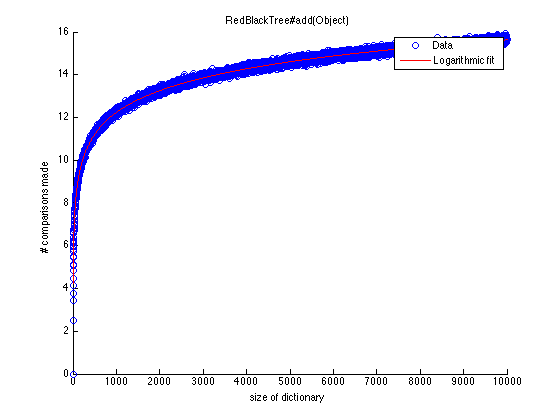
\includegraphics[width=0.49\textwidth]{resources/add}
    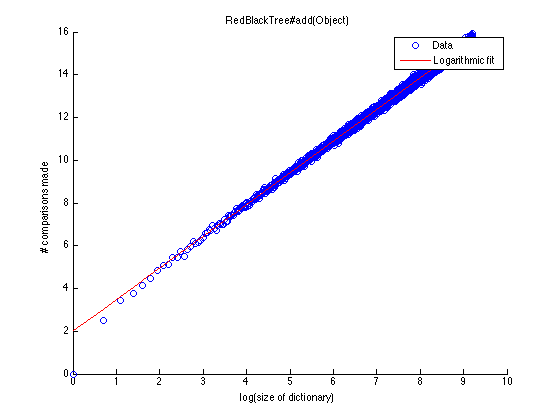
\includegraphics[width=0.49\textwidth]{resources/add_log}
    \caption{The number of comparisons made when adding a random distinct element to a dictionary of size n (linear and log-linear scale)}

\end{figure}

\begin{figure}[!htbp]
    \centering
    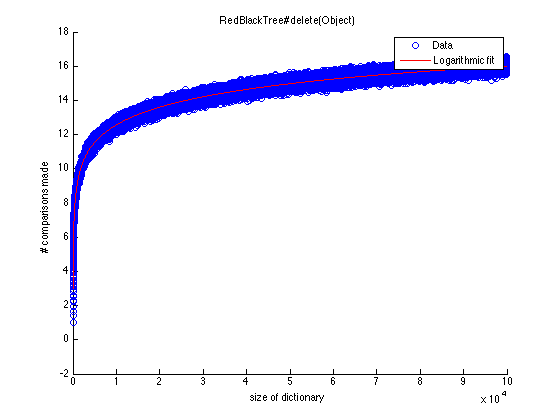
\includegraphics[width=0.49\textwidth]{resources/del}
    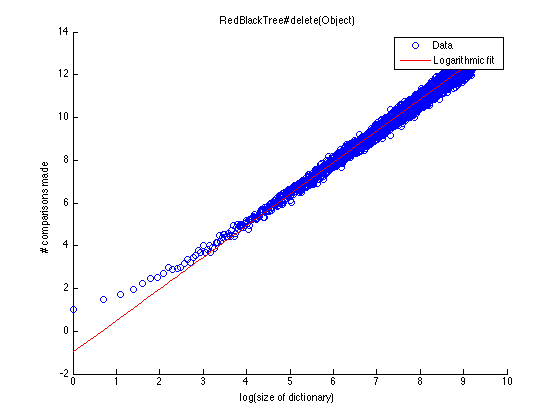
\includegraphics[width=0.49\textwidth]{resources/del_log}
    \caption{The number of comparisons made when deleting a random element from a dictionary of size n (linear and log-linear scale)}
\end{figure}

\begin{figure}[!htbp]
    \centering
    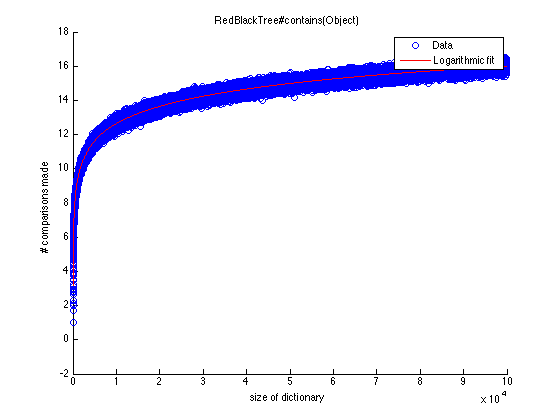
\includegraphics[width=0.49\textwidth]{resources/search}
    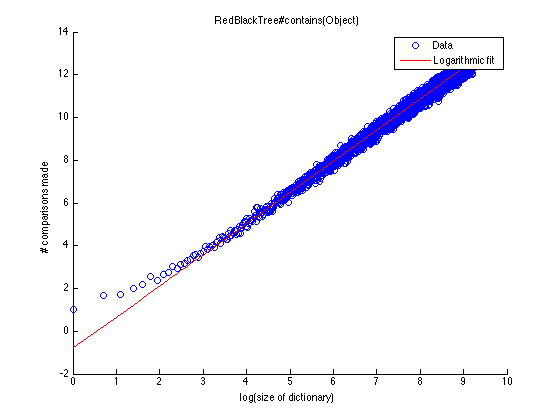
\includegraphics[width=0.49\textwidth]{resources/search_log}
    \caption{The number of comparisons made when searching for a random element in a dictionary of size n (linear and log-linear scale)}
\end{figure}

\begin{table}[!htbp]
\centering
\begin{tabular}{| l | l | l |}
	\hline
	\textbf{Method} & \multicolumn{2}{c |}{\textbf{Comparisons}} \\ \hline
	& \textbf{In dictionary} & \textbf{Not in dictionary} \\ \hline
	\code{isEmpty()} & \multicolumn{2}{l |}{0.0}  \\ \hline
	\code{contains(Object)} & 12.6 & 13.3 \\ \hline
	\code{hasPredecessor(Object)} & \multicolumn{2}{l |}{1.0} \\ \hline
	\code{hasSuccessor(Object)} & \multicolumn{2}{l |}{1.0}  \\ \hline
	\code{predecessor(Object)} & 13.5 & 13.2 \\ \hline
	\code{successor(Object)} & 13.5 & 13.3 \\ \hline
	\code{min()} & \multicolumn{2}{l |}{0.0}  \\ \hline
	\code{max()} & \multicolumn{2}{l |}{0.0}  \\ \hline
	\code{add(Object)} & 12.5 & 15.3 \\ \hline
	\code{delete(Object)} & 12.5 & 13.4 \\ \hline
	\code{iterator()} & \multicolumn{2}{l |}{0.0} \\ \hline
	\code{iterator(Object)} & 12.4 & 13.2\\ \hline
	\code{toString()} & \multicolumn{2}{l |}{0.0} \\
	\hline
\end{tabular}
\caption{Mean number of comparisons made on a dictionary of 10,000 elements, averaged over 100 trials and split into two columns depending on whether the argument is in the dictionary or not.}
\end{table}

The above table makes sense: the 'search' methods (\code{contains}, \code{successor}, etc.) take 12 or 13 comparisons. \code{add} takes approximately 2-3 more since it also compares the element with the current tree minimum and maximum. The constant time methods (\code{isEmpty}, \code{min}, \code{max}) need no comparisons. \code{iterator(Object)} uses the most comparisons since when finding the least element greater than the argument, it needs to keep track of the current least element and compare it with each new possibility when traversing down a subtree. \code{toString} also technically uses zero comparisons, while still being the slowest method (having to visit all nodes results in linear time).
